\documentclass[12pt,letterpaper,final]{article}\usepackage[]{graphicx}\usepackage[]{xcolor}
% maxwidth is the original width if it is less than linewidth
% otherwise use linewidth (to make sure the graphics do not exceed the margin)
\makeatletter
\def\maxwidth{ %
  \ifdim\Gin@nat@width>\linewidth
    \linewidth
  \else
    \Gin@nat@width
  \fi
}
\makeatother

\definecolor{fgcolor}{rgb}{0.345, 0.345, 0.345}
\newcommand{\hlnum}[1]{\textcolor[rgb]{0.686,0.059,0.569}{#1}}%
\newcommand{\hlstr}[1]{\textcolor[rgb]{0.192,0.494,0.8}{#1}}%
\newcommand{\hlcom}[1]{\textcolor[rgb]{0.678,0.584,0.686}{\textit{#1}}}%
\newcommand{\hlopt}[1]{\textcolor[rgb]{0,0,0}{#1}}%
\newcommand{\hlstd}[1]{\textcolor[rgb]{0.345,0.345,0.345}{#1}}%
\newcommand{\hlkwa}[1]{\textcolor[rgb]{0.161,0.373,0.58}{\textbf{#1}}}%
\newcommand{\hlkwb}[1]{\textcolor[rgb]{0.69,0.353,0.396}{#1}}%
\newcommand{\hlkwc}[1]{\textcolor[rgb]{0.333,0.667,0.333}{#1}}%
\newcommand{\hlkwd}[1]{\textcolor[rgb]{0.737,0.353,0.396}{\textbf{#1}}}%
\let\hlipl\hlkwb

\usepackage{framed}
\makeatletter
\newenvironment{kframe}{%
 \def\at@end@of@kframe{}%
 \ifinner\ifhmode%
  \def\at@end@of@kframe{\end{minipage}}%
  \begin{minipage}{\columnwidth}%
 \fi\fi%
 \def\FrameCommand##1{\hskip\@totalleftmargin \hskip-\fboxsep
 \colorbox{shadecolor}{##1}\hskip-\fboxsep
     % There is no \\@totalrightmargin, so:
     \hskip-\linewidth \hskip-\@totalleftmargin \hskip\columnwidth}%
 \MakeFramed {\advance\hsize-\width
   \@totalleftmargin\z@ \linewidth\hsize
   \@setminipage}}%
 {\par\unskip\endMakeFramed%
 \at@end@of@kframe}
\makeatother

\definecolor{shadecolor}{rgb}{.97, .97, .97}
\definecolor{messagecolor}{rgb}{0, 0, 0}
\definecolor{warningcolor}{rgb}{1, 0, 1}
\definecolor{errorcolor}{rgb}{1, 0, 0}
\newenvironment{knitrout}{}{} % an empty environment to be redefined in TeX

\usepackage{alltt}

%\usepackage{Sweave}
\usepackage{graphicx}
\usepackage{natbib}
\usepackage{hyperref}
\usepackage{caption}
\usepackage{rotating}
\usepackage{verbatim}
\usepackage{textcomp}
\usepackage{wasysym}

\setlength{\oddsidemargin}{0in}
\setlength{\textwidth}{6.15in}
%\setlength{\topmargin}{0.5in}
\setlength{\textheight}{22cm}
\setlength{\headheight}{0in}
\setlength{\headsep}{0in}
\setlength{\parskip}{5pt plus 2pt minus 3pt}

\def\thefootnote{\fnsymbol{footnote}}
\setcounter{footnote}{1}

\renewcommand{\baselinestretch}{1.2}
\renewcommand{\labelenumi}{(\roman{enumi})}

\renewcommand{\topfraction}{1.0}
\renewcommand{\bottomfraction}{1.0}
\renewcommand{\textfraction}{0.0}
\renewcommand{\floatpagefraction}{1.0}

\newtheorem{definition}{Definition}
\newtheorem{theorem}{Theorem}
\newtheorem{lemma}[theorem]{Lemma}
\newtheorem{claim}[theorem]{Claim}
\newtheorem{fact}[theorem]{Fact}

% to get nice proofs ...
\newcommand{\qedsymb}{\mbox{ }~\hfill~{\rule{2mm}{2mm}}}
\newenvironment{proof}{\begin{trivlist}
\item[\hspace{\labelsep}{\bf\noindent Proof: }]
}{\qedsymb\end{trivlist}}


\newfont{\msymb}{cmsy10 scaled 1000}

\def\nullset{\mbox{\O}}
\def\R{{I\!\!R}}
\def\C{{I\!\!\!\!C}}
\def\N{{I\!\!N}}

\def\P{\mbox{\msymb P}}


%\parskip 0.1in
\pagenumbering{arabic}    %  Start using 1,2,... as page numbers.
\pagestyle{plain}         %  Page numbers in middle bottom of page.
%\setcounter{page}{80}  % XXXXXXXXXXXXXXXXX
%\setcounter{theorem}{5} % XXXXXXXXXXXXXXXXX
%\setcounter{definition}{10} % XXXXXXXXXXXXXXXXX

\parindent 0in
\IfFileExists{upquote.sty}{\usepackage{upquote}}{}
\begin{document}






\begin{table}\centering
\begin{tabular*}{6.15in}{@{\extracolsep{\fill}}|llr|} \hline
Stat 5050: Introduction to R \\
 & & \\
\multicolumn{3}{|c|}{
{\bf Name:} Peter Kurtz} \\
 & & \\
\multicolumn{3}{|c|}{
Homework Assignment 04} \\
 & & \\
\multicolumn{3}{|c|}{
70 Points } \\
\hline
\end{tabular*}
\end{table}


{\bf General Instructions}

For this fourth homework assignment, you have to work with RMarkdown or knitr/Sweave.
You can create your own RMarkdown (.Rmd) file,
based on files from class and from Homework 1, copy the
question numbers and the answer options into your .Rmd file, 
and knit that file into a pdf file. 
{\bf Alternatively} (and much easier!!!), use this .Rnw file as a 
template, just fill in the answers into the provided spaces,
and knit into a pdf file.

Only the final resulting pdf file (from .Rmd or .Rnw) has to be submitted via Canvas.
As previously stated, I would like to encourage potential and current MS and PhD students
to work with .Rnw and \LaTeX\ instead of .Rmd.

You need to learn how to write R code that is easily readable for others. There exists the
{\it Google's R Style Guide} (provided as a pdf here in Canvas)
that summarizes rules for good R style. 
This style guide closely resembles the far more detailed
{\it Tidyverse Style Guide}.
These rules
are accessible at
\url{https://style.tidyverse.org/}.
In particular, make sure that you always have a space after a comma and that you
consistently use the same type of assignment operator, ideally \verb|<-|.
Look at the examples in these style guides and follow that style whenever you
write your own R code from now on.

{\bf Do not forget to replace my name and include your name instead!}

{\bf In all question parts, show your R code and the results!}

 
 
\newpage


\begin{enumerate}

\item (20 Points) {\bf Family Data Revisited:} \\
In the following exercises, try to write your code to be as general as possible
so that it would still work if the family had 27 members in it or if the 
variables were in a different order in the data frame.

{\bf Show your R code and the final results produced from within R
for all question parts!}


\begin{enumerate}
\item (3 Points)
Copy the family data set for this homework from Canvas into your local folder for this homework.
Then load the \verb|hw04_familyDF.rda| data set into R. Show the ``objects'' that have been loaded.

Is the first ``object'' that is listed a data frame? The R output should be TRUE or FALSE.
Search for help if you don't recall how
to check whether something is a data frame.

\underline{Answer:}
\begin{knitrout}
\definecolor{shadecolor}{rgb}{0.969, 0.969, 0.969}\color{fgcolor}\begin{kframe}
\begin{alltt}
\hlkwd{load}\hlstd{(}\hlstr{'hw04_familyDF.rda'}\hlstd{)}
\hlkwd{names}\hlstd{(family)}
\end{alltt}
\begin{verbatim}
## [1] "firstName" "gender"    "age"       "height"   
## [5] "weight"    "bmi"       "overWt"
\end{verbatim}
\begin{alltt}
\hlkwd{is.data.frame}\hlstd{(family[}\hlnum{1}\hlstd{])}
\end{alltt}
\begin{verbatim}
## [1] TRUE
\end{verbatim}
\end{kframe}
\end{knitrout}


\item (4 Points)
The NHANES survey used different cut-off values for men and women when classifying
them as overweight.  Suppose that a man is classified as obese if his bmi exceeds 26
and a woman is classified as obese if her bmi exceeds 25.
Write a logical expression to create a logical vector, called OW.NHANES, that is TRUE if 
a member of the family is obese and FALSE otherwise. Display its content.

\underline{Answer:}
\begin{knitrout}
\definecolor{shadecolor}{rgb}{0.969, 0.969, 0.969}\color{fgcolor}\begin{kframe}
\begin{alltt}
\hlstd{OW.NHAMES} \hlkwb{=} \hlstd{family[}\hlstr{"bmi"}\hlstd{]} \hlopt{>} \hlnum{25} \hlopt{&} \hlstd{family[}\hlstr{"gender"}\hlstd{]} \hlopt{==} \hlstr{"f"} \hlopt{|}
  \hlstd{family[}\hlstr{"bmi"}\hlstd{]} \hlopt{>} \hlnum{26} \hlopt{&} \hlstd{family[}\hlstr{"gender"}\hlstd{]} \hlopt{==} \hlstr{"m"}
\hlstd{OW.NHAMES}
\end{alltt}
\begin{verbatim}
##         bmi
##  [1,] FALSE
##  [2,] FALSE
##  [3,] FALSE
##  [4,] FALSE
##  [5,] FALSE
##  [6,]  TRUE
##  [7,]  TRUE
##  [8,] FALSE
##  [9,]  TRUE
## [10,]  TRUE
## [11,]  TRUE
## [12,] FALSE
## [13,] FALSE
## [14,] FALSE
\end{verbatim}
\end{kframe}
\end{knitrout}


\item (4 Points)
Here is an alternative way to create the same vector that introduces 
some useful functions and ideas.
We first create a numeric vector called OW.limit that is 26 for each male in
the family and 25 for each female in the family. To do this, we create a vector 
of length 2, called OW.val, where the first element is 26 and second element is 25.
Then we create the OW.limit vector by subsetting OW.val by position, where the 
positions are the numeric values in the gender variable 
(i.e., use as.numeric to coerce the factor vector to a numeric vector).
Notice that we can ``subset'' a vector of length 2 by a much longer vector:

\begin{knitrout}
\definecolor{shadecolor}{rgb}{0.969, 0.969, 0.969}\color{fgcolor}\begin{kframe}
\begin{alltt}
\hlcom{# Note that this code chunk is not executed because eval=FALSE.}
\hlcom{# Change to eval=TRUE once you have answered the previous question parts.}

\hlstd{OW.val} \hlkwb{<-} \hlnum{26}\hlopt{:}\hlnum{25}
\hlstd{OW.limit} \hlkwb{<-} \hlstd{OW.val[}\hlkwd{as.numeric}\hlstd{(family}\hlopt{$}\hlstd{gender)]}
\hlstd{OW.limit}
\end{alltt}
\begin{verbatim}
##  [1] 26 25 26 26 25 25 26 25 26 26 25 26 26 25
\end{verbatim}
\end{kframe}
\end{knitrout}

Finally, use OW.limit and the bmi vector in family to create the desired logical vector, 
and call it OW.NHANES2. Display its content.
Compare with your results from part (b) via the \verb|any| function.
Did you get the intended result? If not, check your R code again!

\underline{Answer:}
\begin{knitrout}
\definecolor{shadecolor}{rgb}{0.969, 0.969, 0.969}\color{fgcolor}\begin{kframe}
\begin{alltt}
\hlstd{OW.NHANES2} \hlkwb{=} \hlstd{family[}\hlstr{"bmi"}\hlstd{]} \hlopt{>=} \hlstd{OW.limit}
\hlstd{OW.NHANES2}
\end{alltt}
\begin{verbatim}
##         bmi
##  [1,] FALSE
##  [2,] FALSE
##  [3,] FALSE
##  [4,] FALSE
##  [5,] FALSE
##  [6,]  TRUE
##  [7,]  TRUE
##  [8,] FALSE
##  [9,]  TRUE
## [10,]  TRUE
## [11,]  TRUE
## [12,] FALSE
## [13,] FALSE
## [14,] FALSE
\end{verbatim}
\begin{alltt}
\hlkwd{setequal}\hlstd{(OW.NHAMES, OW.NHANES2)}
\end{alltt}
\begin{verbatim}
## [1] TRUE
\end{verbatim}
\end{kframe}
\end{knitrout}


\item (4 Points)
Use the vector OW.limit and each person's height to find the weight 
that they would have if their bmi was right at the limit (26 for men and 
25 for women). Call this weight OW.weight and display its content.
To do this, start with the formula \\
\verb|      bmi = (weight / 2.2) / (2.54 / 100 * height)^2| \\
and re-express it in terms of weight (i.e., \verb|weight = ...|).

\underline{Answer:}
\begin{knitrout}
\definecolor{shadecolor}{rgb}{0.969, 0.969, 0.969}\color{fgcolor}\begin{kframe}
\begin{alltt}
\hlstd{heightFam} \hlkwb{=} \hlstd{family[,}\hlkwd{c}\hlstd{(}\hlstr{"height"}\hlstd{)]}
\hlstd{OW.weight} \hlkwb{=} \hlstd{OW.limit}\hlopt{*}\hlstd{(}\hlnum{2.54}\hlopt{/}\hlnum{100}\hlopt{*}\hlstd{heightFam)}\hlopt{**}\hlnum{2}\hlopt{*}\hlnum{2.2}
\hlstd{OW.weight}
\end{alltt}
\begin{verbatim}
##  [1] 180.8254 145.3416 196.6569 165.6582 145.3416 164.0771
##  [7] 170.6402 149.9191 170.6402 186.0288 159.2868 160.7501
## [13] 160.7501 136.3997
\end{verbatim}
\end{kframe}
\end{knitrout}


\item (5 Points)
Create the following plot of actual weight (on the vertical axis)
against the weight at which they would be overweight (on the horizontal axis).
If you get an error when you run this code, check whether you are using
the correct variable names in your code earlier on.

\begin{knitrout}
\definecolor{shadecolor}{rgb}{0.969, 0.969, 0.969}\color{fgcolor}\begin{kframe}
\begin{alltt}
\hlcom{# Note that this code chunk is not executed because eval=FALSE.}
\hlcom{# Change to eval=TRUE once you have answered the previous question parts.}
\hlcom{#}
\hlcom{# Make sure that your graph appears in your output!}

\hlkwd{plot}\hlstd{(OW.weight, family}\hlopt{$}\hlstd{weight,}
     \hlkwc{xlab} \hlstd{=} \hlstr{"Minimum Weight for Overweight"}\hlstd{,}
     \hlkwc{xlim} \hlstd{=} \hlkwd{c}\hlstd{(}\hlnum{100}\hlstd{,} \hlnum{220}\hlstd{),} \hlcom{# !!!}
     \hlkwc{ylab} \hlstd{=} \hlstr{"Observed Weight"}\hlstd{,}
     \hlkwc{ylim} \hlstd{=} \hlkwd{c}\hlstd{(}\hlnum{100}\hlstd{,} \hlnum{220}\hlstd{))} \hlcom{# !!!}

\hlkwd{abline}\hlstd{(}\hlkwc{a} \hlstd{=} \hlnum{0}\hlstd{,} \hlkwc{b} \hlstd{=} \hlnum{1}\hlstd{)}
\end{alltt}
\end{kframe}
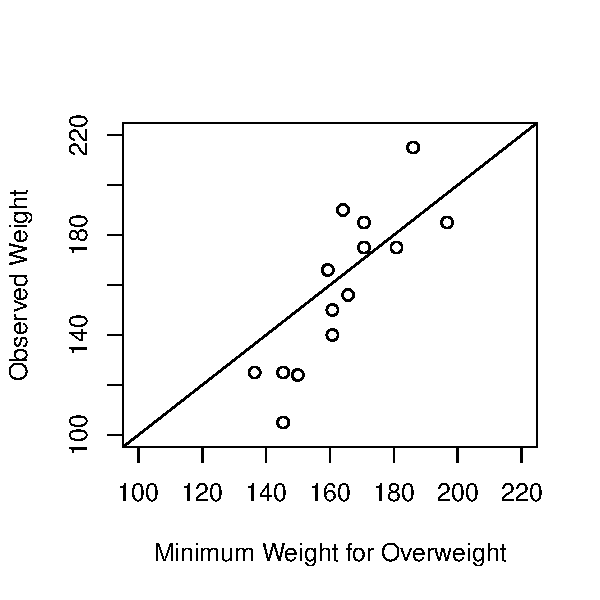
\includegraphics[width=\maxwidth]{figure/unnamed-chunk-7-1} 
\end{knitrout}


\verb|abline| adds a straight line (here with y-intercept $a = 0$ and slope $b = 1$) to the plot.
Note that this is not the regression line!
Thus, points that fall exactly on the line belong to individuals where the observed
weight exactly qualifies to be overweight. Points above the line represent
individuals who are overweight, and points below the line represent
individuals who are not overweight.

{\bf We can easily count in the plot how many points are above the line and how many
points are below the line, but we want that R does this counting for us! 
So, write two R expressions that do this counting for us and display their results.}

\underline{Answer:}
\begin{knitrout}
\definecolor{shadecolor}{rgb}{0.969, 0.969, 0.969}\color{fgcolor}\begin{kframe}
\begin{alltt}
\hlcom{# Number of points above the line}
\hlstd{overWeight} \hlkwb{=} \hlkwd{sum}\hlstd{(OW.NHAMES)}
\hlstd{overWeight}
\end{alltt}
\begin{verbatim}
## [1] 5
\end{verbatim}
\begin{alltt}
\hlcom{# Number of points below the line}
\hlstd{notOverWeight} \hlkwb{=} \hlkwd{length}\hlstd{(OW.NHAMES)} \hlopt{-} \hlstd{overWeight}
\hlstd{notOverWeight}
\end{alltt}
\begin{verbatim}
## [1] 9
\end{verbatim}
\end{kframe}
\end{knitrout}

\end{enumerate}


\newpage


\item (34 Points) {\bf San Francisco Housing Data:} \\
In this question, you have to work with actual housing data from the San Francisco area.

{\bf Show your R code and the final results produced from within R
for all question parts!}

\begin{enumerate}
\item (4 Points)
Copy the San Francisco housing data set (\verb|hw04_SFhousing.rda|) for this homework 
from Canvas into your local folder for this homework.
Then load this data set into R. Show the ``objects'' that have been loaded.
Are cities and housing both data frames? 
Let R answer this question!
The R output should be
TRUE or FALSE for each of these.
Search for help if you don't recall how
to check whether something is a data frame. \\

\underline{Answer:}
\begin{knitrout}
\definecolor{shadecolor}{rgb}{0.969, 0.969, 0.969}\color{fgcolor}\begin{kframe}
\begin{alltt}
\hlkwd{load}\hlstd{(}\hlstr{'hw04_SFHousing.rda'}\hlstd{)}
\hlkwd{names}\hlstd{(housing)}
\end{alltt}
\begin{verbatim}
##  [1] "county"  "city"    "zip"     "street"  "price"  
##  [6] "br"      "lsqft"   "bsqft"   "year"    "date"   
## [11] "long"    "lat"     "quality" "match"   "wk"
\end{verbatim}
\begin{alltt}
\hlkwd{is.data.frame}\hlstd{(housing[}\hlnum{2}\hlstd{])}
\end{alltt}
\begin{verbatim}
## [1] TRUE
\end{verbatim}
\begin{alltt}
\hlkwd{is.data.frame}\hlstd{(housing)}
\end{alltt}
\begin{verbatim}
## [1] TRUE
\end{verbatim}
\end{kframe}
\end{knitrout}


\item (2 Points)
What are the names of the vectors in housing? \\

\underline{Answer:}
\begin{knitrout}
\definecolor{shadecolor}{rgb}{0.969, 0.969, 0.969}\color{fgcolor}\begin{kframe}
\begin{alltt}
\hlkwd{names}\hlstd{(housing)}
\end{alltt}
\begin{verbatim}
##  [1] "county"  "city"    "zip"     "street"  "price"  
##  [6] "br"      "lsqft"   "bsqft"   "year"    "date"   
## [11] "long"    "lat"     "quality" "match"   "wk"
\end{verbatim}
\end{kframe}
\end{knitrout}


\item (2 Points)
How many observations (i.e., rows) are in housing? Only report the number of rows,
but not the number of columns! \\

\underline{Answer:}
\begin{knitrout}
\definecolor{shadecolor}{rgb}{0.969, 0.969, 0.969}\color{fgcolor}\begin{kframe}
\begin{alltt}
\hlkwd{nrow}\hlstd{(housing)}
\end{alltt}
\begin{verbatim}
## [1] 281506
\end{verbatim}
\end{kframe}
\end{knitrout}


\item (6 Points)
Explore the housing data using the summary function. 
Describe in words at least three problems that you see with the data. \\

\underline{Answer:}
{\scriptsize
% I am using \scriptsize to reduce the font size as this output may
% cover a few pages
\begin{knitrout}
\definecolor{shadecolor}{rgb}{0.969, 0.969, 0.969}\color{fgcolor}\begin{kframe}
\begin{alltt}
\hlkwd{summary}\hlstd{(housing)}
\end{alltt}
\begin{verbatim}
##                  county                 city       
##  Santa Clara County :70424   Oakland      : 14730  
##  Alameda County     :60410   Santa Rosa   :  9917  
##  Contra Costa County:59381   Fremont      :  9414  
##  Solano County      :23404   San Francisco:  8137  
##  San Mateo County   :22558   Evergreen    :  7947  
##  Sonoma County      :21676   Antioch      :  7726  
##  (Other)            :23653   (Other)      :223635  
##       zip            street              price         
##  94565  :  4595   Length:281506      Min.   :   22000  
##  94509  :  4302   Class :character   1st Qu.:  400000  
##  95123  :  4023   Mode  :character   Median :  530000  
##  95687  :  3652                      Mean   :  602000  
##  94533  :  3472                      3rd Qu.:  700000  
##  (Other):261457                      Max.   :20000000  
##  NA's   :     5                                        
##        br            lsqft               bsqft        
##  Min.   :1.000   Min.   :       19   Min.   :    122  
##  1st Qu.:2.000   1st Qu.:     4000   1st Qu.:   1121  
##  Median :3.000   Median :     5760   Median :   1430  
##  Mean   :3.024   Mean   :    65939   Mean   :   1624  
##  3rd Qu.:4.000   3rd Qu.:     7701   3rd Qu.:   1882  
##  Max.   :8.000   Max.   :418611600   Max.   :1868120  
##                  NA's   :21687       NA's   :426      
##       year           date                       
##  Min.   :   0   Min.   :2003-04-27 01:00:00.00  
##  1st Qu.:1954   1st Qu.:2004-02-08 01:00:00.00  
##  Median :1971   Median :2004-10-24 01:00:00.00  
##  Mean   :1966   Mean   :2004-11-01 17:06:12.50  
##  3rd Qu.:1985   3rd Qu.:2005-07-24 01:00:00.00  
##  Max.   :3894   Max.   :2006-06-04 01:00:00.00  
##  NA's   :9202                                   
##       long             lat       
##  Min.   :-123.6   Min.   :36.98  
##  1st Qu.:-122.3   1st Qu.:37.50  
##  Median :-122.1   Median :37.77  
##  Mean   :-122.1   Mean   :37.78  
##  3rd Qu.:-121.9   3rd Qu.:38.00  
##  Max.   :-121.5   Max.   :38.85  
##  NA's   :23316    NA's   :23316  
##                                       quality      
##  QUALITY_ADDRESS_RANGE_INTERPOLATION      :170719  
##  gpsvisualizer                            : 31084  
##  QUALITY_CITY_CENTROID                    : 20473  
##  QUALITY_EXACT_PARCEL_CENTROID            : 17208  
##  QUALITY_ZIP_CODE_TABULATION_AREA_CENTROID: 14980  
##  (Other)                                  :  3726  
##  NA's                                     : 23316  
##               match              wk            
##  Exact           :197044   Min.   :2003-04-21  
##  Relaxed         : 30570   1st Qu.:2004-02-01  
##  Relaxed; Soundex: 23338   Median :2004-10-18  
##  Soundex         :  2573   Mean   :2004-10-26  
##  1               :  2244   3rd Qu.:2005-07-18  
##  (Other)         :  2421   Max.   :2006-05-29  
##  NA's            : 23316
\end{verbatim}
\end{kframe}
\end{knitrout}
}

\
\underline{Problems:}
\begin{enumerate}
\item There are many NA values for some of the variables. For example, there is no zip code 
for 5 values, no lsqft for 21687 values, no bsqft for 426, no year for 9202 etc. 
\item The year variable has a minimum of 0 and a maximum of 3894. These are not valid years.
\item This is more of a subjective critique but I think the variable names should be more descriptive. For example, I do not understand what the bf variable is suppose to be. 
\end{enumerate}


\item (4 Points)
Motivated by a historic map from 1938, accessible at
\url{https://www.davidrumsey.com/luna/servlet/detail/RUMSEY~8~1~248517~5515942:Map-of-Oakland,-Berkeley,-Alameda,-},
we will work with houses in the 7 nearby cities of Albany, Alameda, Berkeley, 
Emeryville, Oakland, Piedmont, and San Leandro, only.
Subset the data frame so that we have only houses in these 7 cities,
and keep only the variables city, zip, price, br, bsqft, and year.
Call this new data frame BerkArea. This data frame should have 25,151 observations
and 6 variables (check it!). \\

\underline{Answer:}
\begin{knitrout}
\definecolor{shadecolor}{rgb}{0.969, 0.969, 0.969}\color{fgcolor}\begin{kframe}
\begin{alltt}
\hlstd{chooseVars} \hlkwb{=} \hlkwd{c}\hlstd{(}\hlstr{"city"}\hlstd{,} \hlstr{"zip"}\hlstd{,} \hlstr{"price"}\hlstd{,} \hlstr{"br"}\hlstd{,} \hlstr{"bsqft"}\hlstd{,} \hlstr{"year"}\hlstd{)}
\hlstd{nearCitiesVec} \hlkwb{=} \hlkwd{c}\hlstd{(}\hlstr{"Albany"}\hlstd{,} \hlstr{"Alameda"}\hlstd{,} \hlstr{"Berkeley"}\hlstd{,} \hlstr{"Emeryville"}\hlstd{,} \hlstr{"Oakland"}\hlstd{,} \hlstr{"Piedmont"}\hlstd{,} \hlstr{"San Leandro"}\hlstd{)}
\hlstd{ind} \hlkwb{=} \hlstd{(housing}\hlopt{$}\hlstd{city} \hlopt \hlstd{nearCitiesVec)}
\hlstd{BerkArea} \hlkwb{=} \hlstd{housing[ind,chooseVars]}
\hlkwd{nrow}\hlstd{(BerkArea)}
\end{alltt}
\begin{verbatim}
## [1] 25151
\end{verbatim}
\end{kframe}
\end{knitrout}


\item (4 Points)
We are interested in studying the relationship between price and size of house, but first
we will further subset the data frame to remove the unusually large values.
Use the quantile function to determine the 98th percentile of price and bsqft
and eliminate all of those houses that are above either of these 98th percentiles.
Call this new data frame BerkArea, as well. It should have 24,346 observations (check it!).
Write your code so that it is very general and does not depend on the 
actual numeric value for these quantiles. \\

\underline{Answer:}
\begin{knitrout}
\definecolor{shadecolor}{rgb}{0.969, 0.969, 0.969}\color{fgcolor}\begin{kframe}
\begin{alltt}
\hlstd{quantile95P} \hlkwb{=} \hlkwd{quantile}\hlstd{(BerkArea}\hlopt{$}\hlstd{price,} \hlnum{.98}\hlstd{)}
\hlstd{indQ} \hlkwb{=} \hlstd{BerkArea[}\hlstr{"price"}\hlstd{]} \hlopt{<} \hlstd{quantile95P}

\hlstd{quantile95Q} \hlkwb{=} \hlkwd{quantile}\hlstd{(BerkArea}\hlopt{$}\hlstd{bsqft,} \hlnum{.98}\hlstd{,} \hlkwc{na.rm}\hlstd{=}\hlnum{TRUE}\hlstd{)}
\hlstd{indBs} \hlkwb{=} \hlstd{BerkArea[}\hlstr{"bsqft"}\hlstd{]} \hlopt{<} \hlstd{quantile95Q}

\hlstd{indCom} \hlkwb{=} \hlstd{indQ} \hlopt{&} \hlstd{indBs}

\hlstd{BerkArea}\hlkwb{=}\hlstd{BerkArea[indCom,]}
\hlkwd{nrow}\hlstd{(BerkArea)}
\end{alltt}
\begin{verbatim}
## [1] 24346
\end{verbatim}
\end{kframe}
\end{knitrout}


\item (2 Points)
Create a new vector that is called pricepsqft by dividing the sale price by the square footage
of the house.  Add this new variable to the BerkArea housing data frame
and verify that it indeed has been added to the data frame. \\

\underline{Answer:}
\begin{knitrout}
\definecolor{shadecolor}{rgb}{0.969, 0.969, 0.969}\color{fgcolor}\begin{kframe}
\begin{alltt}
\hlstd{pricepsqft} \hlkwb{=} \hlstd{BerkArea}\hlopt{$}\hlstd{price} \hlopt{/} \hlstd{BerkArea}\hlopt{$}\hlstd{bsqft}
\hlstd{BerkArea}\hlopt{$}\hlstd{pricepsqft} \hlkwb{<-} \hlstd{pricepsqft}
\hlkwd{names}\hlstd{(BerkArea)}
\end{alltt}
\begin{verbatim}
## [1] "city"       "zip"        "price"      "br"        
## [5] "bsqft"      "year"       "pricepsqft"
\end{verbatim}
\end{kframe}
\end{knitrout}


\item (4 Points)
Create a vector called br6 that contains the number of bedrooms in the house, except
when this number is greater than 6, it is set to 6.  That is, if a house has 6 or more
bedrooms then br6 will be 6. Otherwise it will be the number of bedrooms in the house.
Note that there is no need for any ``if''-statements or loops to create this vector ---
just basic R expressions discussed so far will be sufficient! Recall how 
TRUE and FALSE are represented numerically or how to reassign a different value to a subset! \\

\underline{Answer:}
\begin{knitrout}
\definecolor{shadecolor}{rgb}{0.969, 0.969, 0.969}\color{fgcolor}\begin{kframe}
\begin{alltt}
\hlstd{seven} \hlkwb{<-} \hlstd{BerkArea}\hlopt{$}\hlstd{br} \hlopt{>=} \hlnum{7}
\hlstd{eight} \hlkwb{<-} \hlstd{BerkArea}\hlopt{$}\hlstd{br} \hlopt{>=} \hlnum{8}

\hlstd{br6} \hlkwb{<-} \hlstd{BerkArea}\hlopt{$}\hlstd{br} \hlopt{-} \hlstd{seven} \hlopt{-} \hlstd{eight}
\hlstd{BerkArea}\hlopt{$}\hlstd{br6} \hlkwb{<-} \hlstd{br6}
\end{alltt}
\end{kframe}
\end{knitrout}


\item (6 Points)
Recreate the following plot on your side. Then answer the question below.
If you get an error when you run this code, check whether you are using
the correct variable names in your code earlier on.

\begin{knitrout}
\definecolor{shadecolor}{rgb}{0.969, 0.969, 0.969}\color{fgcolor}\begin{kframe}
\begin{alltt}
\hlcom{# Note that this code chunk is not executed because eval=FALSE.}
\hlcom{# Change to eval=TRUE once you have answered the previous question parts.}
\hlcom{#}
\hlcom{# Make sure that your graph appears in your output!}

\hlstd{rCols} \hlkwb{<-} \hlkwd{rainbow}\hlstd{(}\hlnum{6}\hlstd{,} \hlkwc{alpha} \hlstd{=} \hlnum{0.25}\hlstd{)}
\hlstd{brCols} \hlkwb{<-} \hlstd{rCols[br6]}

\hlkwd{plot}\hlstd{(pricepsqft} \hlopt{~} \hlstd{bsqft,} \hlkwc{data} \hlstd{= BerkArea,}
     \hlkwc{main} \hlstd{=} \hlstr{"Housing Prices in the Berkeley Area"}\hlstd{,}
     \hlkwc{xlab} \hlstd{=} \hlstr{"Size of house (square ft)"}\hlstd{,}
     \hlkwc{ylab} \hlstd{=} \hlstr{"Price per square foot"}\hlstd{,}
     \hlkwc{col} \hlstd{= brCols,} \hlkwc{pch} \hlstd{=} \hlnum{19}\hlstd{,} \hlkwc{cex} \hlstd{=} \hlnum{0.5}\hlstd{)}
\hlkwd{legend}\hlstd{(}\hlkwc{legend} \hlstd{=} \hlnum{1}\hlopt{:}\hlnum{6}\hlstd{,} \hlkwc{fill} \hlstd{= rCols,} \hlstr{"topright"}\hlstd{)}
\end{alltt}
\end{kframe}
\end{knitrout}

{\bf What interesting feature do you see in the relationship between these variables that you may not have known before making this plot? 
Numerically quantify (use only 3 decimal digits!) and interpret this feature! HINT: If you aren't sure what measure to use, try searching via google (you should find a 3-letter function in R to calculate this measure of association).} \\

\underline{Answer:} \\
Place your answer here
The relationship between size of house and price per square foot is slightly negative. Also, not surprisingly, the more rooms there are, the bigger the house. Using the correlation function in r outputs a 1.000. This is clearly not correct. Most likely do to something I don't understand or an error. 

\end{enumerate}


\newpage


\item (16 Points) {\bf Survival of Passengers on the Titanic:} \\
Work with the \verb|Titanic| data set, a 4--dimensional array related
to the survival of passengers and crew on board of the Titanic ocean liner.
For further details, refer to the help page via \verb|?Titanic|.
Technically, the Titanic data set is a table, but we can access it similar
to a multi--dimensional array.

{\bf Show your R code and the final results produced from within R
for all question parts!}

\begin{enumerate}
\item (4 Points)
Write an R expression that extracts the numbers of males in all three classes (but not crew)
who survived the sinking of the Titanic. Provide data for children and adults.
The result should look as follows:
\begin{verbatim}
     Age
Class Child Adult
  1st     5    57
  2nd    11    14
  3rd    13    75
\end{verbatim}

\underline{Answer:}
\begin{knitrout}
\definecolor{shadecolor}{rgb}{0.969, 0.969, 0.969}\color{fgcolor}\begin{kframe}
\begin{alltt}
\hlstd{classNotCrew} \hlkwb{<-} \hlkwd{c}\hlstd{(}\hlstr{"1st"}\hlstd{,} \hlstr{"2nd"}\hlstd{,} \hlstr{"3rd"}\hlstd{)}
\hlstd{Titanic[classNotCrew,}\hlkwc{Sex} \hlstd{=} \hlstr{"Male"}\hlstd{,,}\hlkwc{Survived} \hlstd{=} \hlstr{"Yes"}\hlstd{]}
\end{alltt}
\begin{verbatim}
##      Age
## Class Child Adult
##   1st     5    57
##   2nd    11    14
##   3rd    13    75
\end{verbatim}
\end{kframe}
\end{knitrout}


\item (4 Points)
Write an R expression that extracts the numbers of female crew members (adults only)
who survived or did not survive the sinking of the Titanic. 
The result should be a vector of length 2. \\

\underline{Answer:}
\begin{knitrout}
\definecolor{shadecolor}{rgb}{0.969, 0.969, 0.969}\color{fgcolor}\begin{kframe}
\begin{alltt}
\hlstd{Titanic[}\hlkwc{Class} \hlstd{=} \hlstr{"Crew"}\hlstd{,} \hlkwc{Sex} \hlstd{=} \hlstr{"Female"}\hlstd{,} \hlkwc{Age} \hlstd{=} \hlstr{"Adult"}\hlstd{,]}
\end{alltt}
\begin{verbatim}
##  No Yes 
##   3  20
\end{verbatim}
\end{kframe}
\end{knitrout}


\item (4 Points)
Write an R expression that extracts the following matrix from the Titanic data set:
\begin{verbatim}
      Sex
Class  Female Male
  Crew      3  670
  1st       4  118
  2nd      13  154
  3rd      89  387
\end{verbatim}
{\bf Describe what this matrix represents, i.e., which subgroup(s) from the Titanic 
passengers and crew.} \\

\underline{Answer:}
\begin{knitrout}
\definecolor{shadecolor}{rgb}{0.969, 0.969, 0.969}\color{fgcolor}\begin{kframe}
\begin{alltt}
\hlstd{Titanic[,,} \hlkwc{Age} \hlstd{=} \hlstr{"Adult"}\hlstd{,}\hlkwc{Survived}\hlstd{=}\hlstr{"No"}\hlstd{]}
\end{alltt}
\begin{verbatim}
##       Sex
## Class  Male Female
##   1st   118      4
##   2nd   154     13
##   3rd   387     89
##   Crew  670      3
\end{verbatim}
\end{kframe}
\end{knitrout}

\underline{Description:} \\
Place your answer here
The subgroup is Adults that did not survive. 

\item (4 Points)
Write an R expression that extracts the following vector from the Titanic data set:
\begin{verbatim}
[1]  13 14 75 76
\end{verbatim}
{\bf Describe what this vector represents, i.e., which subgroup(s) from the Titanic 
passengers and crew.}
Hint: I first extracted a matrix and then transformed this into a 
vector using \verb|as.vector|. \\

\underline{Answer:}
\begin{knitrout}
\definecolor{shadecolor}{rgb}{0.969, 0.969, 0.969}\color{fgcolor}\begin{kframe}
\begin{alltt}
\hlkwd{as.vector}\hlstd{(}\hlkwd{c}\hlstd{(Titanic[}\hlkwc{Class}\hlstd{=}\hlstr{"3rd"}\hlstd{, ,}\hlkwc{Age}\hlstd{=}\hlstr{"Child"}\hlstd{,} \hlkwc{Survived} \hlstd{=} \hlstr{"Yes"}\hlstd{],}
            \hlstd{Titanic[}\hlkwc{Class}\hlstd{=}\hlstr{"3rd"}\hlstd{, ,}\hlkwc{Age}\hlstd{=}\hlstr{"Adult"}\hlstd{,} \hlkwc{Survived} \hlstd{=} \hlstr{"Yes"}\hlstd{]))}
\end{alltt}
\begin{verbatim}
## [1] 13 14 75 76
\end{verbatim}
\end{kframe}
\end{knitrout}

\underline{Description:} \\
Place your answer here
The first first two are male and female children in the third class that survived. The second two are the same but adults.

\end{enumerate}


\end{enumerate}


\end{document}

